\section{Vorwort}
Bei der Recherche zur Bearbeitung der Übungen wurden viele englischsprachige Webseiten zu rate gezogen. Generell kann man sagen, dass englische Fachbegriffe sich im Bereich FPGA und embedded Design etabliert haben, so dass eine Übersetzung eher verwirren als helfen würde. Daher haben wir uns entschieden, die \textbf{englischen} Bezeichner und Beschreibungen beizubehalten.\\
Um Codeabschnitte besser von Beschreibungen besser unterscheiden zu können, wurde eine eigene Schriftart verwendet:
\begin{verbatim}
  Kommandozeilen Eingaben und Codesnippets werden wie HIER dargestellt.
\end{verbatim}

\section{Aufgabe 1} \label{ex1}
In der Laborübung wurde das ZedBoard Zynq-7000 eingesetzt. Es umfasst als \textbf{PL} den Artix-7 FPGA mit 85K Logic Cells (Device Z-7020, Part: XC7Z020) und als \textbf{PS} den Dual-core ARM Cortex-A9 MPCore™ mit 866 MHz.

\begin{minipage}{\textwidth}
    \begin{center}        
        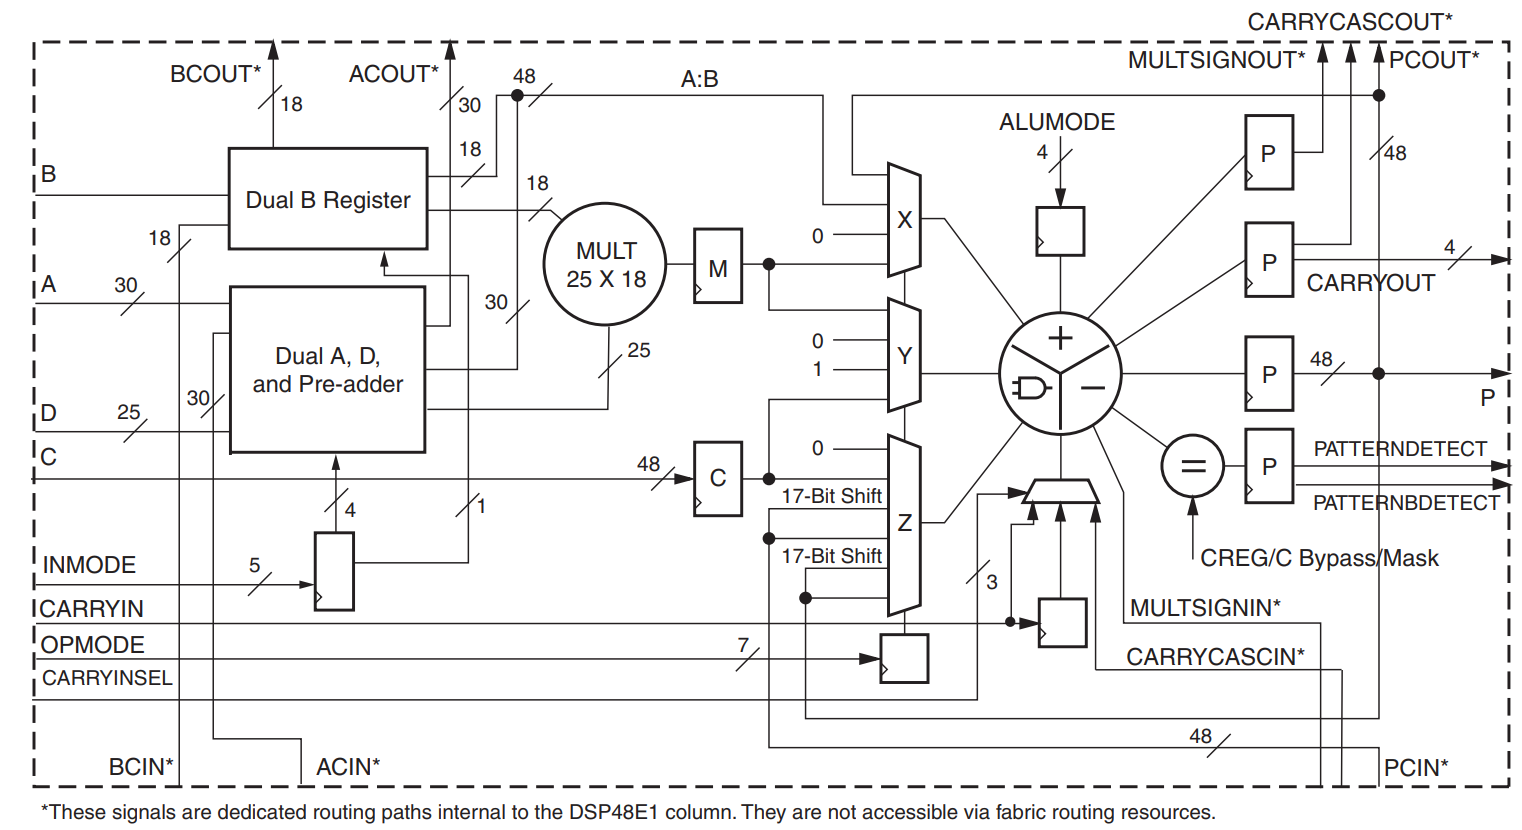
\includegraphics[scale=0.5]{img/DSP48e.png} 
    \end{center}
\end{minipage}
\begin{center}
ZedBoard mit Xilinx Zynq-7000 SoC
\end{center}

Wichtigste Anschlüsse für Laborübung 1
\begin{itemize}
\item b) Netzanschluss
\item c) USB-JTAG (Programmierung)
\item s) USB-UART (serielle Schnittstelle)
\item g) \textbf{VGA-Port} (Display)
\item i) Jumper (Konfiguration eines Programmierungsanschlusses )
\end{itemize}

\subsection {VGA-Controller Theorie}
Die Aufgabe bestand darin einen VGA-Controller in VHDL Entities zu entwickeln. Das Schaubild zeigt die Strukturierung 
des Blockdesigns. Der rot umrandete Block war eigenständig zu entwerfen und zu implementieren. \\
\begin{minipage}{\textwidth}
    \begin{center}        
        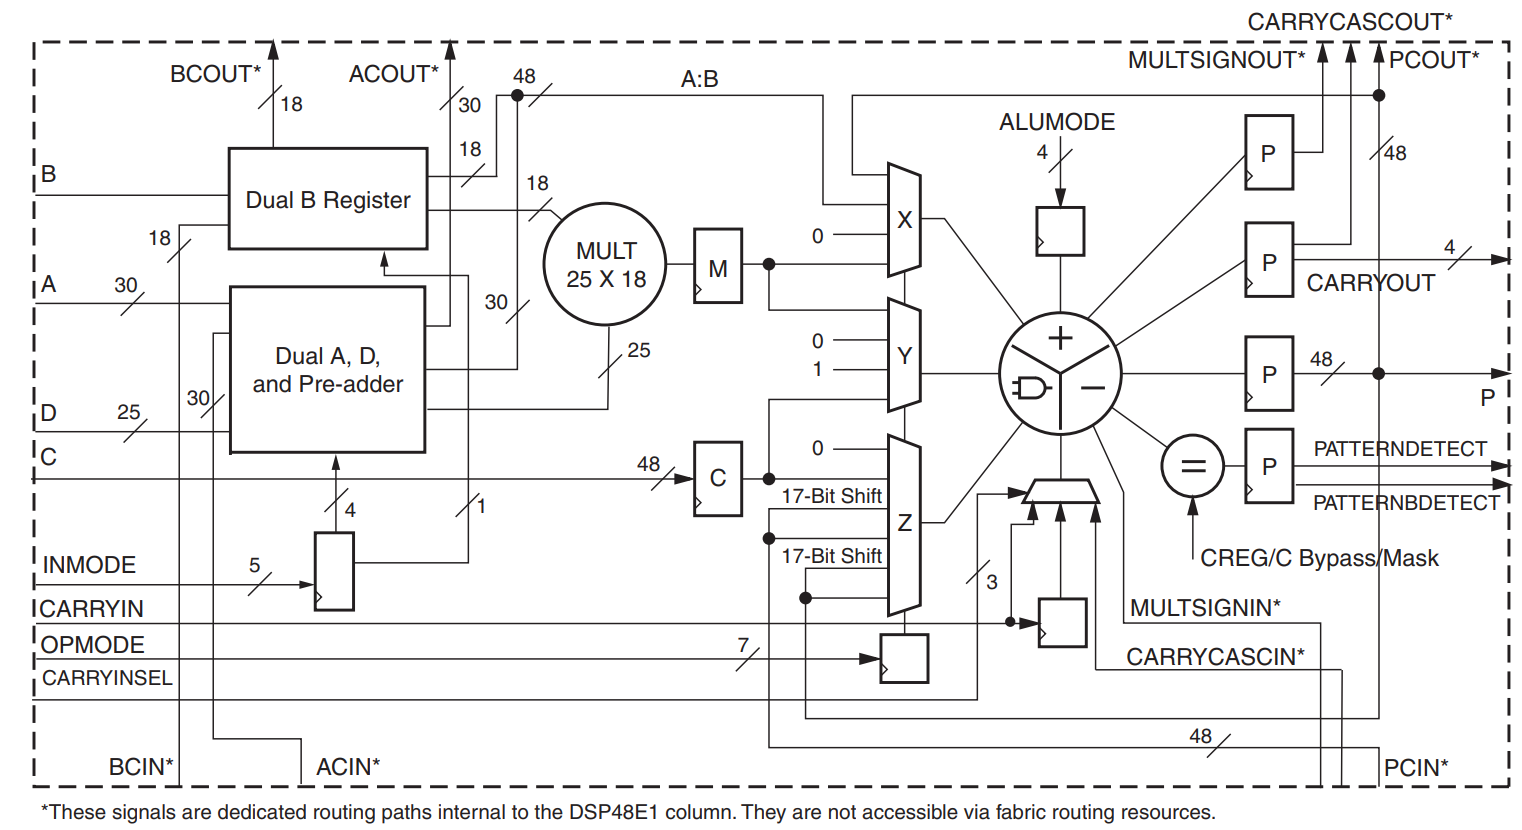
\includegraphics[scale=0.5]{img/DSP48e.png} 
    \end{center}
\end{minipage}
\begin{center}
VGA Controller Schema
\end{center}

\begin{minipage}{\textwidth}
    \begin{center}        
        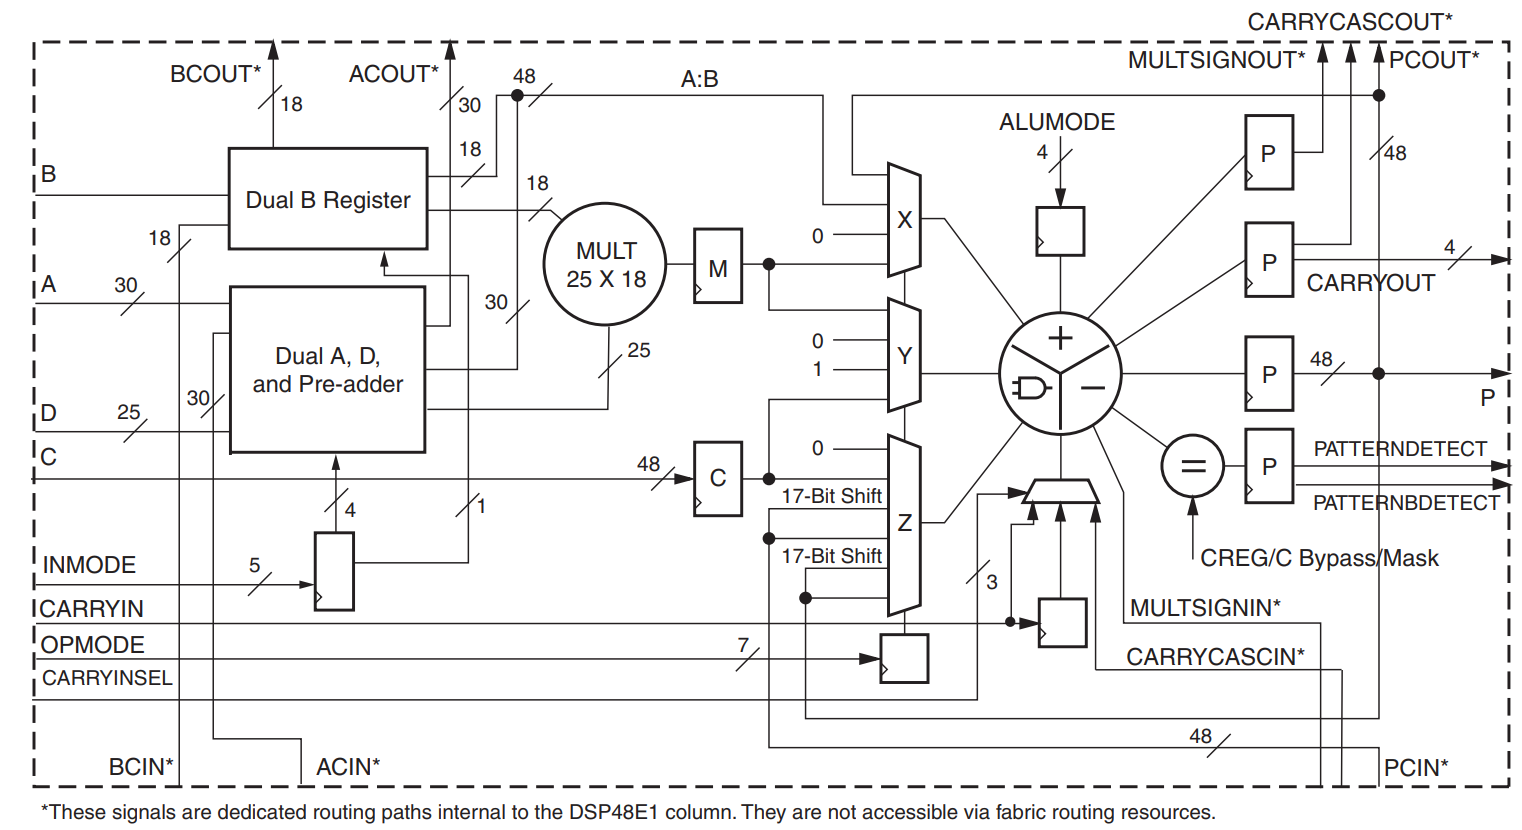
\includegraphics[scale=0.5]{img/DSP48e.png} 
    \end{center}
\end{minipage}
\begin{center}
VGA Portbelegung
\end{center}

Das VGA-Signal besteht aus dem sichtbaren Bildbereich. Hier 640*480px und dem Front- und Backporch Bereich, der in vergangener 
Zeit dazu diente den Elektronenstrahl zu lenken. Insgesamt sind inklusive aller Bereiche 800*525 mit dem VGA-Signal zu takten.\\
Um die Clock-Geschwindigkeit zu berechnen wird eine Bildaufbaufrequnz von 60Hz angestrebt. \\
800*525*60 = 25,2 M Pixel/s.\\

\begin{minipage}{\textwidth}
    \begin{center}        
        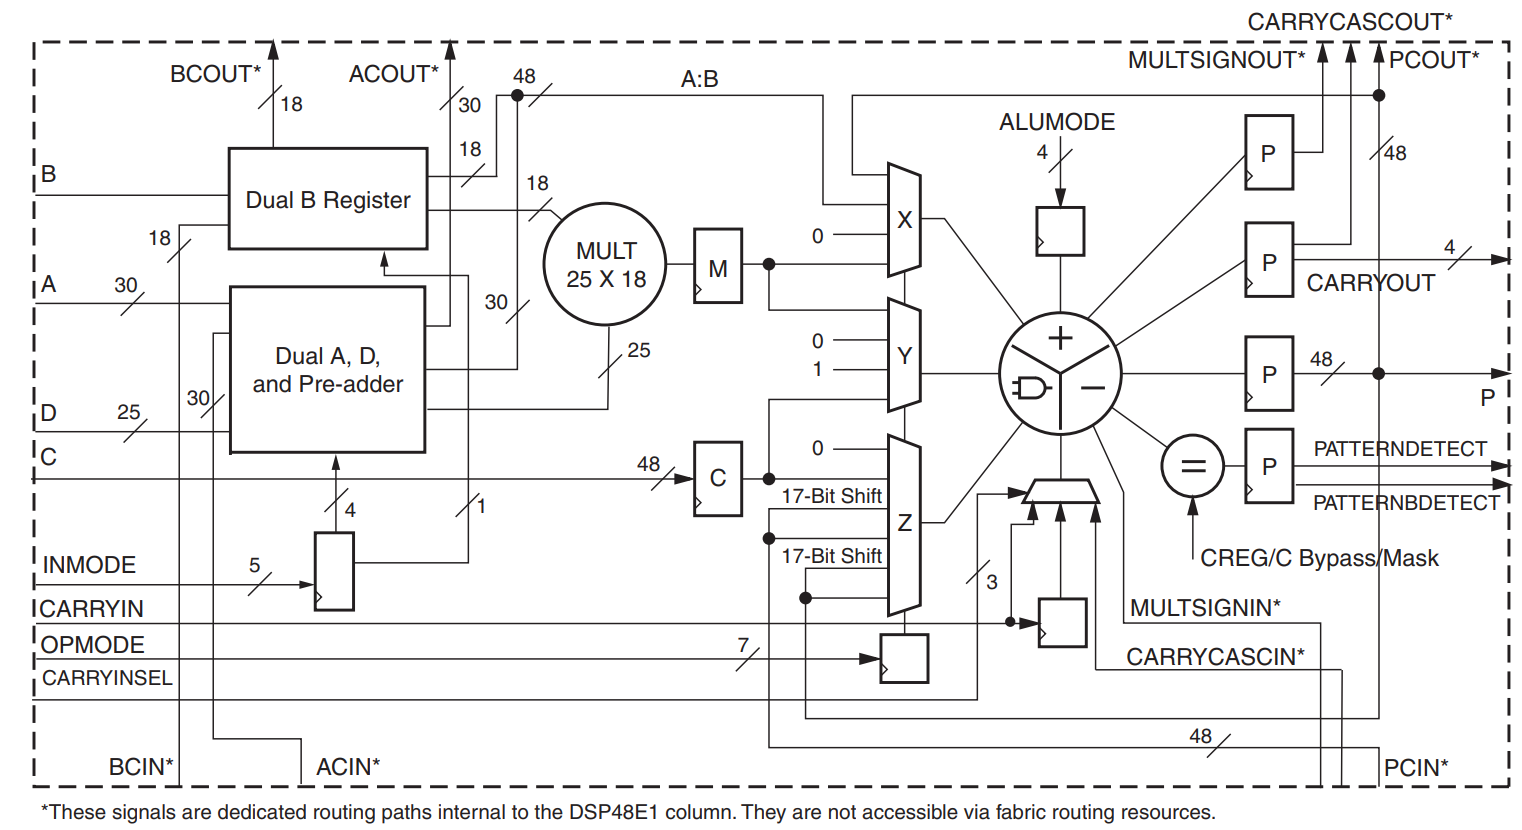
\includegraphics[scale=0.5]{img/DSP48e.png} 
    \end{center}
\end{minipage}
\begin{center}
VGA Bildbereich und Porches
\end{center}

\subsection{VGA-Controller Implementation}
Hier wird das Vivado Block Diagramm dargestellt, mit sys\_clock im unteren rechten Bereich (100MHz) so wie dem clk\_wtz\_0 um 
die Clock auf 25.172 MHz zu reduzieren. Der util\_vector\_logic\_0 negiert das locked Signal und kann so als Reset Signal für die VGA\_Controller verwendet werden.\\

\begin{minipage}{\textwidth}
    \begin{center}        
        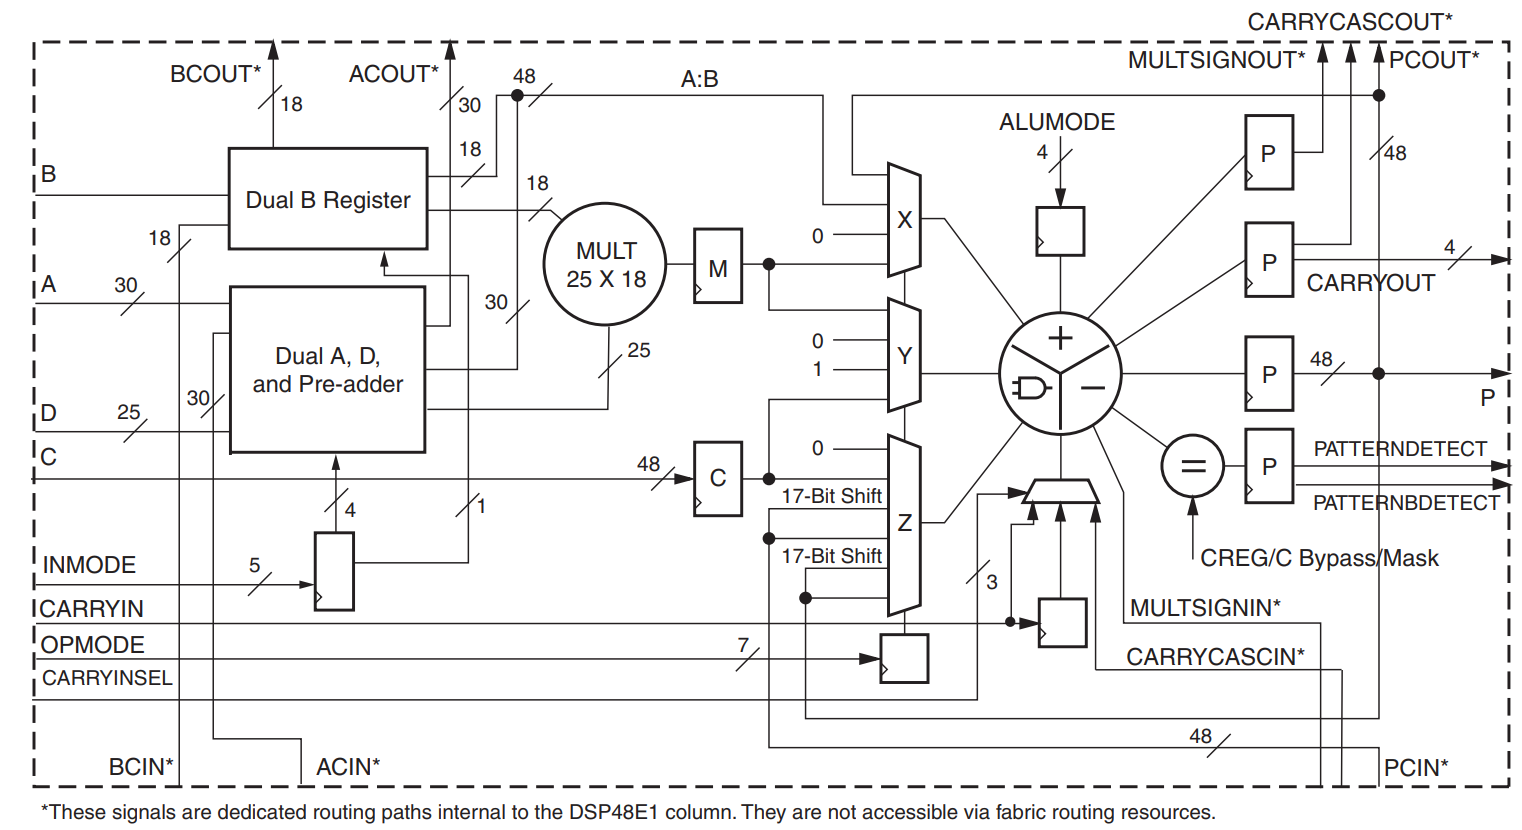
\includegraphics[scale=0.5]{img/DSP48e.png} 
    \end{center}
\end{minipage}
\begin{center}
Vivado Blockdiagramm
\end{center}

Als Beispielanzeige der Simulation mit den Testdaten (reduzierte Bildgröße) wurde ein  Bereich imunteren Porch-Bereich ausgewählt. Sobald vsync `0' ist werden die Pixelzähler wieder auf (0,0) für den nächsten Frame zurückgesetzt. Die zwei rund markierten Signalbereiche stellen die hsync Signale dar, die auch gesetzt werden, wenn das vsync Signal `0' ist. \\

\begin{minipage}{\textwidth}
    \begin{center}        
        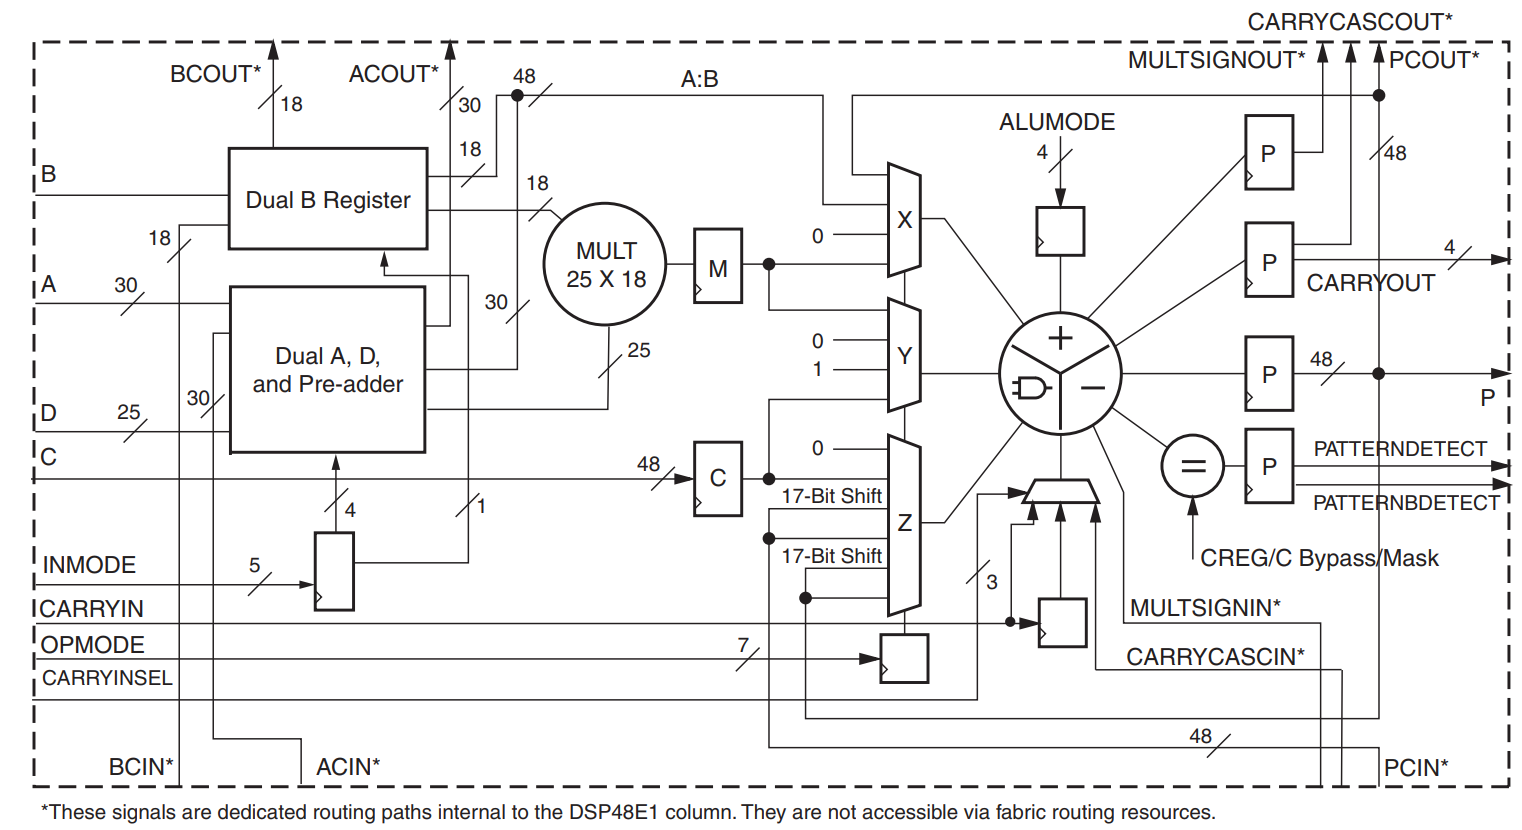
\includegraphics[scale=0.4]{img/DSP48e.png} 
    \end{center}
\end{minipage}
\begin{center}
Vivado Simulation
\end{center}

Vivado Ports für die Bank 33 (3.3V), je 4 Signale gehen an die Farbkanäle und nur zwei hsync und vsync kontrollieren 
die Zeilen und Spalten.\\

\begin{minipage}{\textwidth}
    \begin{center}
        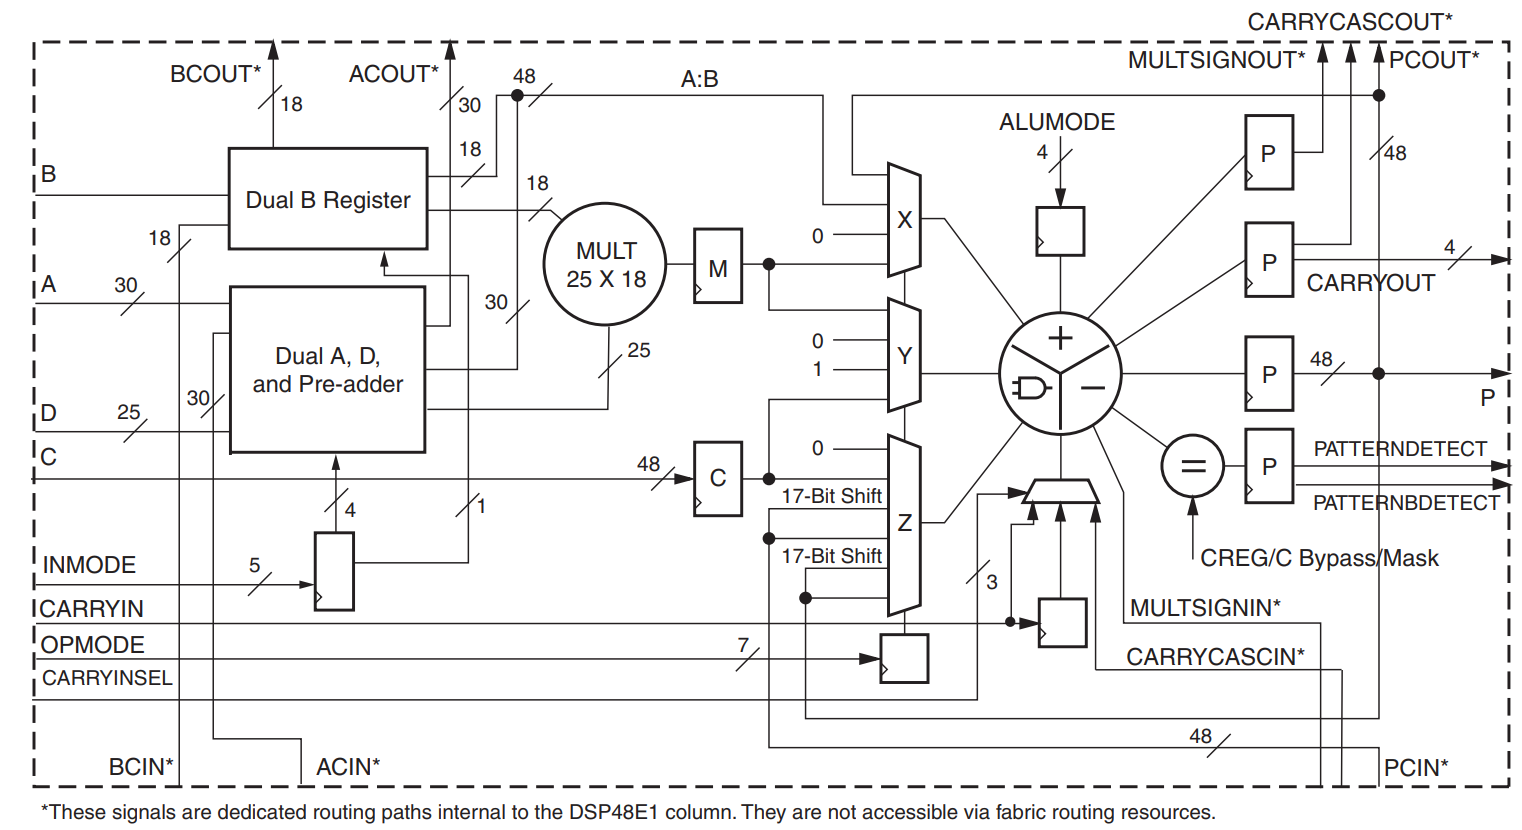
\includegraphics[scale=0.6]{img/DSP48e.png} 
    \end{center}
\end{minipage}
\begin{center}
VGA Port Belegung Vivado
\end{center}


vga\_sync Entity:
\begin{verbatim}
 ----------------------------------------------------------------------------------
-- Create Date: 09.12.2018 12:48:58
-- Module Name: vga_sync - impl
----------------------------------------------------------------------------------
library ieee;
use ieee.std_logic_1164.all;
use ieee.numeric_std.all;

-- Uncomment the following library declaration if using
-- arithmetic functions with Signed or Unsigned values
--use IEEE.NUMERIC_STD.ALL;

-- Uncomment the following library declaration if instantiating
-- any Xilinx leaf cells in this code.
--library UNISIM;
--use UNISIM.VComponents.all;

entity vga_sync is
    Port ( vga_clk   : in  std_logic;
           reset     : in  std_logic;
           pixel_x   : out std_logic_vector (9 downto 0);
           pixel_y   : out std_logic_vector (9 downto 0);
           video_on  : out std_logic;
           hSync     : out std_logic;
           vSync     : out std_logic);
end vga_sync;

architecture impl of vga_sync is
   -- REAL VGA MONITOR DATA 
    CONSTANT h_active_sig : integer := 799; -- full horizontal
    CONSTANT h_active_video  : integer := 639; -- horizontal active video
    -- CONSTANT h_front_porch : integer := 16; -- horizontal front porch
    -- CONSTANT h_retrace     : integer := 96; --horizontal retrace/sync pulse length
    -- CONSTANT h_back_porch : integer := 48; -- horizontal back porch
    CONSTANT h_retrace  : integer := 655; --h_active_video 639 + 16
    CONSTANT h_back_porch :integer := 752; --h_active_video 639+16+96 (+1 for<check)
    
    CONSTANT v_active_sig : integer := 524; -- full vertical
    CONSTANT v_active_video  : integer := 479; -- vertical active video
    -- CONSTANT v_front_porch : integer := 10; -- vertical front porch
    -- CONSTANT v_retrace  : integer := 2; -- vertical retrace / sync pulse length
    -- CONSTANT v_back_porch : integer := 33; --vertical back porch
    CONSTANT v_retrace  : integer:= 489; -- v_active_video 479 + 10
    CONSTANT v_back_porch :integer:= 492; --v_active_video 479+10+2 (+1 for<check)
   
   -- TEST SIGNALS for SIMULATION -- 
    -- CONSTANT h_active_sig    : integer := 29; -- full horizontal
    -- CONSTANT h_active_video  : integer := 19; -- horizontal active video
    -- -- CONSTANT h_front_porch  : integer := 16; -- horizontal front porch
    -- -- CONSTANT h_retrace :integer := 96; --horizontal retrace/sync pulse length
    -- -- CONSTANT h_back_porch  : integer := 48; -- horizontal back porch
    -- CONSTANT h_retrace : integer := 24; -- h_active_video 639 + 16
    -- CONSTANT h_back_porch :integer := 27; --h_active_video 639+16+96 (+1 for<check)
    -- 
    -- CONSTANT v_active_sig    : integer := 19; -- full vertical
    -- CONSTANT v_active_video  : integer := 9; -- vertical active video
    -- -- CONSTANT v_front_porch   : integer := 10; -- vertical front porch
    -- -- CONSTANT v_retrace : integer := 2; -- vertical retrace/sync pulse length
    -- -- CONSTANT v_back_porch    : integer := 33; -- vertical back porch
    -- CONSTANT v_retrace       : integer := 13; -- v_active_video 479 + 10
    -- CONSTANT v_back_porch : integer := 16; --v_active_video 479+10+2 (+1 for<check)

   signal px_reg   : unsigned(9 downto 0) := (others => '0'); -- x full 0 to 799
   signal px_next  : unsigned(9 downto 0);
   signal py_reg   : unsigned(9 downto 0) := (others => '0'); -- y full 0 to 524
   signal py_next  : unsigned(9 downto 0);
   
   signal hsync_reg  : std_logic := '0';
   signal hsync_next : std_logic;
   
   signal vsync_reg  : std_logic := '0';
   signal vsync_next : std_logic;
   
   signal video_on_reg  : std_logic := '0';
   signal video_on_next : std_logic;
   
begin
   -- IMPLEMENTATION WITH REGISTERS
    vga_count : process (vga_clk)
    begin
        if (rising_edge(vga_clk)) then
            if (reset = '1') then
                px_reg    <= (others => '0');
                py_reg    <= (others => '0');
               
                hsync_reg <= '1';
                vsync_reg <= '1';
            else
            
                -- full size counter including porches
                px_reg  <= px_next;
                py_reg  <= py_next;
                
                -- sync signalss
                hsync_reg <= hsync_next;
                vsync_reg <= vsync_next;
                
                -- video active - inactive
                video_on_reg <= video_on_next;
      
            end if;
        end if;
    end process vga_count;
    
    -- CHECK all REQUIREMENTS for sync and video_on.
    -- modulo 799
    px_next <= (others => '0') when (px_reg = h_active_sig) else px_reg + 1; 
    
    -- reset on h=799 and v=524 (max rows)
    py_next<=(others=>'0') when ((px_reg=h_active_sig) and (py_reg=v_active_sig)) else 
           py_reg + 1  when (px_reg=h_active_sig) else py_reg; -- add 1 if row finished 
    
    -- modulo 639 in col, 479 in row
    video_on_next<='0' when((px_reg>h_active_video) or (py_reg>v_active_video)) else '1'; 
    
     -- '0' from 656 to 751 (96 px)
    hsync_next <= '0' when ((px_reg > h_retrace) and (px_reg < h_back_porch)) else '1';
    -- '0' from 490 to 491 (2 px)
    vsync_next <= '0' when ((py_reg > v_retrace) and (py_reg < v_back_porch)) else '1';  
    
    -- set output from registers
    pixel_x <= std_logic_vector(px_reg);
    pixel_y <= std_logic_vector(py_reg);
    video_on <= video_on_reg;
    hSync    <= hsync_reg;
    vSync    <= vsync_reg;

end impl;
 \end{verbatim}